         \chapter{Skills for science}
    \setcounter{figure}{1}\setcounter{subfigure}{1}\label{m30853}
    \section{Introduction}
            \nopagebreak
In the physical sciences there are many skills that you need to learn. These include working with units, basic mathematics skills and laboratory skills. In this chapter we will revise some of these skills that you should know before starting to study physical science. This chapter is intended as a reference guide to assist you in your journey of studying physical science. 
\section{Mathematical skills}
You should be comfortable with scientific notation and how to write scientific notation. You should also be able to easily convert between different units and change the subject of a formula. In addition, concepts such as rate, direct and indirect proportion, fractions and ratios and the use of constants in equations are important. 
\subsection*{Rounding off}
Certain numbers may take an infinite amount of paper and ink to write out. Not only is that impossible, but writing numbers out to a high precision (many decimal places) is very inconvenient and rarely gives better answers. For this reason we often estimate the number to a certain number of decimal places. \\
Rounding off a decimal number to a given number of decimal places is the quickest way to approximate a number. For example, if you wanted to round-off $2,6525272$ to three decimal places then you would first count three places after the decimal. Next you mark this point with a $|$: $2,652|5272$. All numbers to the right of $|$ are ignored after you determine whether the number in the third decimal place must be rounded up or rounded down. You \textsl{round up} the final digit (make the digit one more) if the first digit after the $|$ is greater than or equal to 5 and \textsl{round down} (leave the digit alone) otherwise. So, since the first digit after the $|$ is a 5, we must round up the digit in the third decimal place to a 3 and the final answer of $2,6525272$ rounded to three decimal places is $2,653$. \\
In a calculation that has many steps, it is best to leave the rounding off right until the end. This ensures that your answer is more accurate.
\subsection*{Scientific notation}
In science one often needs to work with very large or very small numbers. These can be written more easily (and more compactly) in scientific notation, in the general form:       
    \begin{equation*}
    N \times 10^{n}
      \end{equation*}
where $N$ is a decimal number between $0$ and $10$ that is rounded off to a few decimal places. $n$ is known as the \textsl{exponent} and is an integer. If $n\greatthan{}0$ it represents how many times the decimal place in $N$ should be moved to the right. If $n\lessthan{}0$, then it represents how many times the decimal place in $N$ should be moved to the left. For example $3,24\ensuremath{\times}{10}^{3}$ represents $3~240$ (the decimal moved three places to the right) and $3,24\ensuremath{\times}{10}^{-3}$ represents $0,00324$ (the decimal moved three places to the left).\\
If a number must be converted into scientific notation, we need to work out how many times the number must be multiplied or divided by 10 to make it into a number between 1 and 10 (i.e. the value of $n$) and what this number between 1 and 10 is (the value of $N$). We do this by counting the number of decimal places the decimal comma must move.\\
For example, write the speed of light ($299 ~792 ~458 \text{ m} \cdot \text{ s}^{-1}$) in scientific notation, to two decimal places. First, we find where the decimal comma must go for two decimal places (to find $N$) and then count how many places there are after the decimal comma to determine $n$.\\
In this example, the decimal comma must go after the first $2$, but since the number after the $9$ is $7$, $N=3,00$. $n=8$ because there are $8$ digits left after the decimal comma. So the speed of light in scientific notation, to two decimal places is $3,00 \times 10^{8} \text{ m} \cdot \text{s}^{-1}$. \\
We can also perform addition, subtraction, multiplication and division with scientific notation. The following two worked examples show how to do this:
\begin{wex}{Addition and subtraction with scientific notation}
 {$1,99 \times 10^{-26} + 1,67 \times 10^{-27} - 2,79 \times 10^{-25} = ?$}
{\westep{Make all the exponents the same}
To add or subtract numbers in scientific notation we must make all the exponents the same:\\
$1,99 \times 10^{-26} = 0,199 \times 10^{-25}$ and\\
$1,67 \times 10^{-27} = 0,0167 \times 10^{-25}$
\westep{Carry out the addition and subtraction}
Now that the exponents are the same we can simply add or subtract the $N$ part of each number:\\
$0,199 + 0,0167 - 2,79 = -2,5743$ 
\westep{Write the final answer}
To get the final answer we put the common exponent back:\\
$-2,5743 \times 10^{-25}$
}
\end{wex}
Note that we follow the same process if the exponents are positive. For example $5,1 \times 10^{3} + 4,2 \times 10^{4} = 4,71 \times 10^{4}$. 
\begin{wex}{Multiplication and division with scientific notation}
 {$1,6 \times 10^{-19} \times 3,2 \times 10^{-19} \div 5 \times 10^{-21} $}
{ \westep{Carry out the multiplication}
For multiplication and division the exponents do not need to be the same. For multiplication we add the exponents and multiply the $N$ terms:\\
$1,6 \times 10^{-19} \times 3,2 \times 10^{-19} = (1,6 \times 3,2) \times 10^{-19 + (-19)} = 5,12 \times 10^{-38}$
\westep{Carry out the division}
For division we subtract the exponents and divide the $N$ terms. Using our result from the previous step we get:\\
$2,56 \times 10^{-38} \div 5 \times 10^{-21} = (5,12 \div 5) \times 10^{-38 - (-19)} = 1,024 \times 10^{-18}$
\westep{Write the final answer}
The answer is: $1,024 \times 10^{-18}$
}
\end{wex}
Note that we follow the same process if the exponents are positive. For example: $5,1 \times 10^{3} \times 4,2 \times 10^{4} = 21,42 \times 10^{7} = 2,142 \times 10^{8}$
\section{Units}
Imagine you had to make curtains and needed to buy fabric. The shop assistant would need to know how much fabric you needed. Telling her you need fabric 2 wide and 6 long would be insufficient --- you have to specify the \textbf{unit} (i.e. 2 \textsl{meters} wide and 6 \textsl{metros} long). Without the unit the information is incomplete and the shop assistant would have to guess. If you were making curtains for a doll's house the dimensions might be 2 centimetres wide and 6 centimetres long!\\ 
It is not just lengths that have units, all physical quantities have units (e.g. time, temperature, distance, etc.).\\
\Definition{Physical Quantity } { A physical quantity is anything that you can measure. For example, length, temperature, distance and time are physical quantities.} 
There are many different systems of units. The main systems of units are: 
\begin{itemize}
 \item SI units
\item c.g.s units
\item Imperial units
\item Natural units
\end{itemize}
\subsection*{SI Units}
            \nopagebreak
We will be using the SI units in this course. SI units are the internationally agreed upon units. 
 \Definition{ SI Units } { The name \textsl{SI units} comes from the French \textsl{Syst\`{e}me International d'Unit\'{e}s}, which means \textsl{international system of units}.  } 
There are seven base SI units. These are listed in table~\ref{tab:units:SIunits}. All physical quantities have units which can be built from these seven base units. So, it is possible to create a different set of units by defining a different set of base units.\\
These seven units are called base units because none of them can be expressed as combinations of the other six. These base units are like the 26 letters of the alphabet for English. Many different words can be formed by using these letters.\par 
\begin{table}[H]
\centering
\begin{tabular}{|c|c|c|}\hline
\textbf{Base quantity} & \textbf{Name} & \textbf{Symbol} \\
\hline length & meter & m\\ \hline 
mass & kilogram & kg\\ \hline 
time & second & s\\ \hline 
electric current & ampere& A\\ \hline temperature & kelvin & K\\ \hline 
amount of substance & mole & mol\\ \hline 
luminous intensity & candela & cd\\ \hline
\end{tabular}
\caption{SI Base Units}\label{tab:units:SIunits}
\end{table}
 \subsection*{The Other Systems of Units}
            \nopagebreak
The SI Units are not the only units available, but they are most widely used. In Science there are three other sets of units that can also be used. These are mentioned here for interest only.
\begin{itemize}
 \item \textbf{c.g.s. Units} \\
In the c.g.s. system, the meter is replaced by the centimetre and the kilogram is replaced by the gram. This is a simple change but it means that all units derived from these two are changed. For example, the units of force and work are different. These units are used most often in astrophysics and atomic physics.
\item \textbf{Imperial Units} \\
Imperial units arose when kings and queens decided the measures that were to be used in the land. All the imperial base units, except for the measure of time, are different to those of SI units. This is the unit system you are most likely to encounter if SI units are not used. Examples of imperial units are pounds, miles, gallons and yards. These units are used by the Americans and British. As you can imagine, having different units in use from place to place makes scientific communication very difficult. This was the motivation for adopting a set of internationally agreed upon units.
\item \textbf{Natural Units} \\
This is the most sophisticated choice of units. Here the most fundamental discovered quantities (such as the speed of light) are set equal to 1. The argument for this choice is that all other quantities should be built from these fundamental units. This system of units is used in high energy physics and quantum mechanics.
\end{itemize}
% \subsection*{Writing units as words or symbols}
%             \nopagebreak
% Unit names are always written with a lowercase first letter, for example, we write metre and litre. The symbols or abbreviations of units are also written with lowercase initials, for example $m$ for metre and $\ell $ for litre. The exception to this rule is if the unit is named after a person, then the symbol is a capital letter. For example, the kelvin was named after Lord Kelvin and its symbol is K. If the abbreviation of the unit that is named after a person has two letters, the second letter is lowercase, for example Hz for hertz.\par 
\subsection*{Combinations of SI base units}
            \nopagebreak
To make working with units easier, some combinations of the base units are given special names, but it is always correct to reduce everything to the base units. Table~\ref{tab:SIcombinations} lists some examples of combinations of SI base units that are assigned special names. Do not be concerned if the formulae look unfamiliar at this stage - we will deal with each in detail in the chapters ahead (as well as many others)! \\ 
It is very important that you are able to recognise the units correctly. For example, the \textbf{newton} (N) is another name for the \textbf{kilogram meter per second squared} (kg$\ensuremath{\cdot}$m$\ensuremath{\cdot}$s${}^{-2}$), while the \textbf{kilogram meter squared per second squared} (kg$\ensuremath{\cdot}$m${}^{2}\ensuremath{\cdot}$s${}^{-2}$) is called the \textbf{joule} (J).
          \begin{table}[H]
        \begin{center}
\noindent
      \begin{tabular}{|l|l|l|l|}\hline
\textbf{Quantity} & \textbf{Formula} & \textbf{Unit Expressed in Base Units}              & \textbf{Name of Combination} \\ \hline
Force             & $ma$             & $\text{kg}\cdot \text{m} \cdot \text{s}^{-2}$      & N (newton)                   \\ \hline
Frequency         & $\frac{1}{T}$    & $\text{s}^{-1}$                                    & Hz (hertz)                   \\ \hline
Work              & $Fs$             & $\text{kg} \cdot \text{m}^{2} \cdot \text{s}^{-2}$ & J (joule)                    \\ \hline
    \end{tabular}
\caption{Some examples of combinations of SI base units assigned special names}
\label{tab:SIcombinations}
      \end{center}
\end{table}
    \par
\label{m30853*notfhsst!!!underscore!!!id306}
\Tip{When writing combinations of base SI units, place a dot ($\ensuremath{\cdot}$) between the units to indicate that different base units are used. For example, the symbol for meters per second is correctly written as m$\ensuremath{\cdot}$s${}^{-1}$, and not as ms${}^{-1}$ or m/s. Although the last two options will be accepted in tests and exams, we will only use the first one in this book.}
\subsection*{Prefixes of base units}
            \nopagebreak
Now that you know how to write numbers in scientific notation, another important aspect of units is the prefixes that are used with the units. In the case of units, the prefixes have a special use. The kilogram (kg) is a simple example. 1 kg is equal to 1 000 g or $1\ensuremath{\times}{10}^{3}$ g. Grouping the ${10}^{3}$ and the g together we can replace the ${10}^{3}$ with the prefix k (kilo). Therefore the k takes the place of the ${10}^{3}$. The kilogram is unique in that it is the only SI base unit containing a prefix.\\
In science, all the prefixes used with units are some power of 10. Table~\ref{tab:unitprefixes} lists some of these prefixes. You will not use most of these prefixes, but those prefixes listed in \textbf{bold} should be learnt. The case of the prefix symbol is very important. Where a letter features twice in the table, it is written in uppercase for exponents bigger than one and in lowercase for exponents less than one. For example M means mega (10${}^{6}$) and m means milli (10${}^{-3}$).
          \begin{table}[H]
        \begin{center}
    \noindent
      \begin{tabular}{|l|l|l|l|l|l|}\hline
\textbf{Prefix} & \textbf{Symbol}  & \textbf{Exponent} & \textbf{Prefix} & \textbf{Symbol} & \textbf{Exponent} \\ \hline
yotta           & Y                & ${10}^{24}$       & yocto           & y               & ${10}^{-24}$      \\ \hline
zetta           &  Z               & ${10}^{21}$       &  zepto          & z               & ${10}^{-21}$      \\ \hline
exa             &  E               & ${10}^{18}$       & atto            & a               & ${10}^{-18}$      \\ \hline
peta            & P                & ${10}^{15}$       & femto           & f               & ${10}^{-15}$      \\ \hline
tera            &  T               & ${10}^{12}$       &  pico           & p               & ${10}^{-12}$      \\ \hline
\textbf{giga}   & G                & ${10}^{9}$        & \textbf{nano}   & n               & ${10}^{-9}$       \\ \hline
\textbf{mega}   &  M               & ${10}^{6}$        & \textbf{micro}  & $\mu $          & ${10}^{-6}$       \\ \hline
\textbf{kilo}   &  k               & ${10}^{3}$        & \textbf{milli}  & m               & ${10}^{-3}$       \\ \hline
\textbf{hecto}  &  h               & ${10}^{2}$        & \textbf{centi}  & c               & ${10}^{-2}$       \\ \hline
\textbf{deca}   &  da              & ${10}^{1}$        & \textbf{deci}   & d               & ${10}^{-1}$       \\ \hline
    \end{tabular}
\caption{Unit Prefixes}
      \end{center}
\label{tab:unitprefixes}
\end{table}
\Tip{There is no space and no dot between the prefix and the symbol for the unit.}
Here are some examples of the use of prefixes:
\begin{itemize}[noitemsep]
  \item $40~000 \text{ m}$ can be written as $40 \text{ km}$ (kilometre)
  \item $0,001 \text{ g}$ is the same as $1 \times{10}^{-3} \text{ g}$ and can be written as $1 \text{ mg}$ (milligram)
  \item $2,5 \times {10}^{6}$ N can be written as $2,5 \text{ MN}$ (meganewton)
  \item $250~000 \text{ A}$ can be written as $250 \text{ kA}$ (kiloampere) or $0,250 \text{ MA}$ (megaampere)
  \item $0,000000075 \text{ s}$ can be written as $75 \text{ ns}$ (nanoseconds)
  \item $3 \times{10}^{-7} \text{ mol}$ can be rewritten as $0,3 \times{10}^{-6} \text{ mol}$, which is the same as $0,3 ~\mu \text{mol}$ (micromol)
\end{itemize}
\begin{exercises}{Scientific Notation }
            \nopagebreak \noindent
\begin{enumerate}[noitemsep, label=\textbf{\arabic*}. ] 
 \item Carry out the following calculations:
    \begin{enumerate}[noitemsep, label=\textbf{\alph*}. ] 
     \item $1,63 \times 10^{5} + 4,32 \times 10^{6} - 8,53 \times 10^{5}$
     \item $7,43 \times 10^{3} \div 6,54 \times 10^{7} \times 3,33 \times 10^{5}$
     \item $6,21434534 \times 10^{-5} \times 3,2555 \times 10^{-3} + 6,3 \times 10^{-4}$
    \end{enumerate}
  \item Write the following in scientific notation using Table \ref{tab:unitprefixes} as a reference.
    \begin{enumerate}[noitemsep, label=\textbf{\alph*}. ] 
      \item $0,511 \text{ MV}$
      \item $10 \text{ c}\ell $
      \item $0,5 ~\mu\text{m}$
      \item $250 \text{ nm}$
      \item $0,00035 \text{ hg}$
    \end{enumerate}
  \item Write the following using the prefixes in Table \ref{tab:unitprefixes}.
    \begin{enumerate}[noitemsep, label=\textbf{\alph*}. ] 
      \item $1,602 \times{10}^{-19} \text{ C}$
      \item $1,992 \times{10}^{6} \text { J}$
      \item $5,98 \times{10}^{4} \text{ N}$
      \item $25 \times{10}^{-4} \text{ A}$
      \item $0,0075 \times{10}^{6} \text{ m}$
    \end{enumerate}
\end{enumerate}
\par \practiceinfo
 \par \begin{tabular}[h]{cccccc}
(1.) & lDG & (2.) lOR  &  (3.) lOn  & \end{tabular}
\end{exercises}
\subsection*{The Importance of Units}
            \nopagebreak
Without units much of our work as scientists would be meaningless. We need to express our thoughts clearly and units give meaning to the numbers we measure and calculate. Depending on which units we use, the numbers are different. For example if you have 12 water, it means nothing. You could have 12 ml of water, 12 litres of water, or even 12 bottles of water. Units are an essential part of the language we use. Units must be specified when expressing physical quantities. Imagine that you are baking a cake, but the units, like grams and millilitres, for the flour, milk, sugar and baking powder are not specified!
\begin{groupdiscussion}{Importance of Units }
            \nopagebreak
Work in groups of 5 to discuss other possible situations where using the incorrect set of units can be to your disadvantage or even dangerous. Look for examples at home, at school, at a hospital, when travelling and in a shop. 
\end{groupdiscussion}
\begin{casestudy}{The importance of units }
            \nopagebreak
Read the following extract from CNN News 30 September 1999 and answer the questions below.\\
\textbf{NASA: Human error caused loss of Mars orbiter November 10, 1999}\\
Failure to convert English measures to metric values caused the loss of the Mars Climate Orbiter, a spacecraft that smashed into the planet instead of reaching a safe orbit, a NASA investigation concluded Wednesday.\\
The Mars Climate Orbiter, a key craft in the space agency's exploration of the red planet, vanished on 23 September after a 10 month journey. It is believed that the craft came dangerously close to the atmosphere of Mars, where it presumably burned and broke into pieces.\\
An investigation board concluded that NASA engineers failed to convert English measures of rocket thrusts to newton, a metric system measuring rocket force. One English pound of force equals 4,45 newtons. A small difference between the two values caused the spacecraft to approach Mars at too low an altitude and the craft is thought to have smashed into the planet's atmosphere and was destroyed.\\
The spacecraft was to be a key part of the exploration of the planet. From its station about the red planet, the Mars Climate Orbiter was to relay signals from the Mars Polar Lander, which is scheduled to touch down on Mars next month.\\
``The root cause of the loss of the spacecraft was a failed translation of English units into metric units and a segment of ground-based, navigation-related mission software,'' said Arthus Stephenson, chairman of the investigation board.\\
\textbf{Questions:}\\
\begin{enumerate}[noitemsep, label=\textbf{\arabic*}. ] 
\item Why did the Mars Climate Orbiter crash? Answer in your own words.
\item How could this have been avoided?
\item Why was the Mars Orbiter sent to Mars?
\item Do you think space exploration is important? Explain your answer.
\end{enumerate}
\end{casestudy}
\subsection*{How to change units}
            \nopagebreak
It is very important that you are aware that different systems of units exist. Furthermore, you must be able to convert between units. Being able to change between units (for example, converting from millimetres to meters) is a useful skill in Science.\\ 
The following conversion diagrams will help you change from one unit to another.
\setcounter{subfigure}{0}
\begin{figure}[H]
\begin{center}
\scalebox{1} % Change this value to rescale the drawing.
{
\begin{pspicture}(0,-0.97605497)(5.9353123,0.976055)
\usefont{T1}{ptm}{m}{n}
\rput(0.27453125,-0.006054977){mm}
\usefont{T1}{ptm}{m}{n}
\rput(2.9545312,0.013945023){m}
\usefont{T1}{ptm}{m}{n}
\rput(5.664531,-0.006054977){km}
\psbezier[linewidth=0.04,arrowsize=0.05291667cm 2.0,arrowlength=1.4,arrowinset=0.4]{->}(0.296875,-0.15605497)(0.296875,-0.956055)(2.896875,-0.956055)(2.896875,-0.15605497)
\psbezier[linewidth=0.04,arrowsize=0.05291667cm 2.0,arrowlength=1.4,arrowinset=0.4]{->}(3.016875,-0.15605497)(3.016875,-0.956055)(5.616875,-0.956055)(5.616875,-0.15605497)
\usefont{T1}{ptm}{m}{n}
\rput(1.506875,-0.576055){\small $\div$1000}
\usefont{T1}{ptm}{m}{n}
\rput(4.326875,-0.576055){\small $\div$1000}
\usefont{T1}{ptm}{m}{n}
\rput(1.606875,0.50394505){\small $\times$1000}
\usefont{T1}{ptm}{m}{n}
\rput(4.346875,0.50394505){\small $\times$1000}
\psbezier[linewidth=0.04,arrowsize=0.05291667cm 2.0,arrowlength=1.4,arrowinset=0.4]{->}(2.896782,0.23767163)(2.9016154,0.92058134)(0.30180123,0.956055)(0.29696798,0.27314526)
\psbezier[linewidth=0.04,arrowsize=0.05291667cm 2.0,arrowlength=1.4,arrowinset=0.4]{->}(5.636782,0.23767163)(5.6416154,0.92058134)(3.0418012,0.956055)(3.036968,0.27314526)
\end{pspicture} 
}
\end{center}
\caption{The distance conversion table}
\label{ch2:conversion1}
\end{figure}      
If you want to change millimetre to meter, you divide by 1000 (follow the arrow from mm to m); or if you want to change kilometre to millimetre, you multiply by 1000$\ensuremath{\times}$1000.\par 
The same method can be used to change millilitre to lit re or kilolitre. Use Figure~\ref{ch2:conversion2} to change volumes: 
    \setcounter{subfigure}{0}
\begin{figure}[H] % horizontal\label{m30853*uid56}
\begin{center}
\scalebox{1} % Change this value to rescale the drawing.
{
\begin{pspicture}(0,-1.146055)(6.6696873,1.146055)
\usefont{T1}{ptm}{m}{n}
\rput(0.5271875,0.20394503){m$\ell$}
\usefont{T1}{ptm}{m}{n}
\rput(3.3912501,0.20394503){$\ell$}
\usefont{T1}{ptm}{m}{n}
\rput(6.1171875,0.20394503){k$\ell$}
\psbezier[linewidth=0.04,arrowsize=0.05291667cm 2.0,arrowlength=1.4,arrowinset=0.4]{->}(0.6784375,-0.326055)(0.6784375,-1.126055)(3.2784376,-1.126055)(3.2784376,-0.326055)
\psbezier[linewidth=0.04,arrowsize=0.05291667cm 2.0,arrowlength=1.4,arrowinset=0.4]{->}(3.3984375,-0.326055)(3.3984375,-1.126055)(5.9984374,-1.126055)(5.9984374,-0.326055)
\usefont{T1}{ptm}{m}{n}
\rput(1.9684376,-0.706055){\small $\div$1000}
\usefont{T1}{ptm}{m}{n}
\rput(4.6484375,-0.706055){\small $\div$1000}
\usefont{T1}{ptm}{m}{n}
\rput(1.9684376,0.673945){\small $\times$1000}
\usefont{T1}{ptm}{m}{n}
\rput(4.7084374,0.673945){\small $\times$1000}
\psbezier[linewidth=0.04,arrowsize=0.05291667cm 2.0,arrowlength=1.4,arrowinset=0.4]{->}(3.2783444,0.40767163)(3.2831779,1.0905813)(0.6833637,1.126055)(0.6785305,0.44314525)
\psbezier[linewidth=0.04,arrowsize=0.05291667cm 2.0,arrowlength=1.4,arrowinset=0.4]{->}(6.0183444,0.40767163)(6.0231776,1.0905813)(3.4233634,1.126055)(3.4185305,0.44314525)
\usefont{T1}{ptm}{m}{n}
\rput(3.3484375,-0.13605498){dm$^3$}
\usefont{T1}{ptm}{m}{n}
\rput(6.1471877,-0.116054974){m$^3$}
\usefont{T1}{ptm}{m}{n}
\rput(0.54265624,-0.13605498){cm$^3$}
\end{pspicture} 
}
\end{center}
\caption{The volume conversion table}
\label{ch2:conversion2}
 \end{figure}       
\begin{wex}{Conversion 1 }{Express 3 800 mm in meters. }
 {
\westep{Use the conversion table} Use Figure~\ref{ch2:conversion1} . Milli meter is on the left and meter in the middle.
\westep{Decide which direction you are moving}You need to go from mm to m, so you are moving from left to right.
\westep{Write the answer}$3 800 \text{ mm} \div 1~000 = 3,8 \text{ m}$ 
    }
\end{wex}
    \noindent
\par
\begin{wex}{Conversion 2}{Convert 4,56 kg to g.}
{\westep{Find the two units on the conversion diagram.}
Use Figure \ref{ch2:conversion1}. Kilogram is the same as kilometre and gram is the same as meter.\\
\westep{Decide whether you are moving to the left or to the right.}
You need to go from kg to g, so it is from right to left.\\
\westep{Read from the diagram what you must do and find the answer.}
$4,56 \text{ kg} \times 1~000 = 4~560 \text{ g}$}
\end{wex}
\subsubsection*{Two other useful conversions}
            \nopagebreak
Very often in science you need to convert speed and temperature. The following two rules will help you do this:
\begin{enumerate}[label=\textbf{\arabic*}.]
\item \textbf{Converting speed}\\
When converting $\text{km} \cdot \text{h}^{-1}$ to $\text{m} \cdot} \text{s}^{-1}$you divide by $3,6$ ($\dfrac{1000 \text{ m}}{3600 \text{ s}}$). For example $72 \text{ km} \cdot \text{h}^{-1} \div 3,6 = 20 \text{m}\cdot \text{s}^{-1}$.\\  
When converting $\text{m}\cdot} \text{s}^{-1}$ to $\text{km} \cdot \text{h}^{-1}$, you multiply by $3,6$. For example $30 \text{ m}\cdot \text{s}^{-1} \times 3,6 = 108 \text{km} \cdot \text{h}^{-1}$. 
\item \textbf{Converting temperature}\\
Converting between the kelvin and Celsius temperature scales is easy. To convert from Celsius to Kelvin add $273$. To convert from Kelvin to Celsius subtract $273$. Representing the Kelvin temperature by ${T}_{K}$ and the Celsius temperature by ${T}_{^{\circ}C}$:         
    \begin{equation*}
    {T}_{K}={T}_{^{\circ}C} + 273
      \end{equation*}
\subsection*{Changing the subject of a formula}
Very often in science you will have to change the subject of a formula. We will look at two examples. (Do not worry if you do not yet know what the terms and symbols mean, these formulae will be covered later in the book.)
\begin{enumerate}[label=\textbf{\arabic*}.]
 \item \textbf{Moles}\\
The equation to calculate moles from molar mass is: $n = \frac{m}{M}$, where $n$ is the number of moles, $m$ is the mass and $M$ is the molar mass. As it is written we can easily find the number of moles of a substance. But what if we have the number of moles and want to find the molar mass? We note that we can simply multiply both sides of the equation by the molar mass and then divide both sides by the number of moles:
\begin{eqnarray*}
 n & = & \frac{m}{M} \\
nM & = & m \\
M & = & \frac{m}{n}
\end{eqnarray*}
And if we wanted the mass we would use: $m = nM$.
\item \texbf{Energy of a photon}\\
The equation for the energy of a photon is $E = h\frac{c}{\lambda}$, where $E$ is the energy, $h$ is Planck's constant, $c$ is the speed of light and $\lambda$ is the wavelength. To get $c$ we can do the following:
\begin{eqnarray*}
 E & = & h\frac{c}{\lambda} \\
E \lambda & = & hc \\
c & = & \frac{E \lambda}{h}
\end{eqnarray*}  
Similarly we can find the wavelength we use: $\lambda = \frac{hc}{E}$ and to find Planck's constant we use: $h =  \frac{E \lambda}{c}$.
\end{enumerate}
\subsection*{Rate, proportion and ratios}
In science we often want to know how a quantity relates to another quantity or how something changes over a period of time. To do this we need to know about rate, proportion and ratios. \\
\textbf{Rate:}\\
The rate at which something happens is the number of times that it happens over a period of time. The rate is always a change per time unit. So we can get rate of change of velocity per unit time ($\frac{\Delta \vec{v}}{t}$) or the rate of change in concentration per unit time (or $\frac{\Delta{C}}{t}$). (Note that $\Delta$ represents a change in). \\
\textbf{Ratios and fractions:}\\
A fraction is a number which represents a part of a whole and is written as $\frac{a}{b}$, where $a$ is the numerator and $b$ is the denominator. A ratio tells us the relative size of one quantity (e.g. number of moles of reactants) compared to another quantity (e.g. number of moles of product): $2:1$, $4:3$, etc. Ratios can also be written as fractions as percentages (fractions with a denominator of 100). \\
\textbf{Proportion:}\\
Proportion is a way of describing relationships between values or between constants. We can say that $x$ is directly proportional to $y$ ($x \propto y$) or that $a$ is indirectly proportional to $b$ ($a \propto \frac{1}{b}$). It is important to understand the difference between directly and inversely proportional.
\begin{itemize}
 \item \textbf{Directly proportional}\\
Two values or constants are directly proportional when a change in one leads to the same change in the other. This is a more-more relationship. We can represent this as $y \propto x$ or $y = kx$ where $k$ is the proportionality constant. We have to include $k$ since we do not know by how much $x$ changes when $y$ changes. $x$ could change by 2 for every change of 1 in $y$. If we plot two directly proportional variables on a graph, then we get a straight line graph that goes through the origin $(0;0)$:
\\
\scalebox{.6}{
\begin{pspicture}(0,0)(6,6)
\psaxes[linewidth=1pt,labels=none,ticks=none]{->}(0,0)(0,0)(5,5)
\psplot[plotpoints=200]{0}{5}{x}
\end{pspicture}}
 
\item \textbf{Inversely proportional}\\
Two values or constants are indirectly proportional when a change in one leads to the opposite change in the other. We can represent this as $y = \frac{k}{x}$. This is a more-less relationship. If we plot two indirectly proportional variables we get a curve that never cuts the axis:\\
\scalebox{.7} % Change this value to rescale the drawing.
{
\begin{pspicture}(0,-2.8429167)(5.7458334,2.8629167)
\rput(0.74583334,-2.1570833){\psaxes[linewidth=1pt,labels=none,ticks=none]{->}(0,0)(0,0)(5,5)}
\psbezier[linewidth=0.04](0.92583334,2.8429167)(1.1658334,-0.41708332)(0.54583335,-1.8970833)(5.7258334,-1.9770833)
\end{pspicture} 
}
\end{itemize}

\subsection*{Constants in equations}
A constant in an equation \textbf{always} has the same value. For example the speed of light ($c = 2,99 \times 10^{8} \text{ m} \cdot \text{ s}^{-1}$), Planck's constant ($h$) and Avogadro's number ($A$) are all examples of constants that are use in science. The following table lists all the constants that you will encounter in this book.
\begin{table}[H]
 \begin{center}
  \begin{tabular}{|l|l|l|l|}\hline
   \textbf{Constant} & Symbol & \textbf{Units} & \textbf{SI Units} \\ \hline
Atomic mass unit & $u$ & $1,67 \times 10^{-24} \text{ g}$ & $1,67 \times 10^{-27} \text{ kg}$ \\ \hline
Charge on an electron & $e$ & $-1,6 \times 10^{-19} \text{ C}$ & $-1,6 \times 10^{-19} \text{ s}\cdot \text{A}$ \\ \hline
Speed of sound (in air, at $25^{\circ}$) & & \multicolumn{2}{l|}{$344 m \cdot s^{-1}$} \\ \hline
Speed of light & $c$ & \multicolumn{2}{l|}{$3 \times 10^{8} m \cdot s^{-1}$} \\ \hline
Planck's constant & $h$ & $6,626 \times 10^{-34} \text{ J} \cdot \text{s}$ & $6,626 \times 10^{-34} \text{ kg} \cdot \text{m}^{2} \text{s}^{-1}$ \\ \hline
Avogadro's number & $N_{A}$ & \multicolumn{2}{l|}{$6,022 \times 10^{23}$} \\ \hline
Gravitational acceleration & $g$ & \multicolumn{2}{l|}{$9,8 \text{ m} \cdot \text{s}^{-1}$} \\ \hline  
  \end{tabular}
 \end{center}
\end{table}

\subsection*{Trigonometry}
Trigonometry is the relationship between the angles and sides of right angled triangles. Trigonometrical relationships are ratios and therefore have no units. You should know the following trigonometric ratios:
\begin{figure}[H]
 \begin{center}
\scalebox{0.8} % Change this value to rescale the drawing.
{
\begin{pspicture}(0,-1.4227902)(3.3625,1.7750223)
\pspolygon[linewidth=0.04](0.3825,-1.0049777)(0.3825,1.7550223)(3.3425,-1.0049777)
\rput{52.407463}(0.39958495,-2.654173){\psarc[linewidth=0.04](2.896345,-0.92112124){0.5946196}{58.71599}{138.21469}}
\usefont{T1}{ptm}{m}{n}
\rput(2.7290626,-0.77497774){A}
\usefont{T1}{ptm}{m}{n}
\rput(1.7764063,-1.1949778){adjacent}
\usefont{T1}{ptm}{m}{n}
\rput{-45.0}(0.30270198,1.6130193){\rput(2.09625,0.4650223){hypotenuse}}
\usefont{T1}{ptm}{m}{n}
\rput{90.0}(0.20502228,-0.12185272){\rput(0.15125,0.06502228){opposite}}
\end{pspicture} 
}
 \end{center}
\end{figure}

\begin{itemize}
 \item Sine\\
This is defined as $\text{sin} A = \frac{\text{opposite}}{\text{hypotenuse}}$
\item Cosine \\
This is defined as $\text{cos} A = \frac{\text{adjacent}}{\text{hypotenuse}}$
\item Tangent \\
This is defined as $\text{tan} A = \frac{\text{opposite}}{\text{adjacent}}$
\end{itemize}
\begin{exercises}{Using Significant Figures }
            \nopagebreak
\begin{enumerate}[noitemsep, label=\textbf{\arabic*}. ] 
\item Write the following quantities in scientific notation:
\begin{enumerate}[noitemsep, label=\textbf{\alph*}. ] 
\item 10130 Pa to 2 decimal places
\item 978,15 m$\ensuremath{\cdot}$s${}^{-2}$ to one decimal place
\item 0,000001256 A to 3 decimal places
\end{enumerate}
\item For each of the following symbols, write out the unit in full and write what power of 10 it represents:
  \begin{enumerate}[noitemsep, label=\textbf{\alph*}. ] 
  \item $\mu $g
  \item mg
  \item kg
  \item Mg
  \end{enumerate}
\item Write each of the following in scientific notation, correct to 2 decimal places:
  \begin{enumerate}[noitemsep, label=\textbf{\alph*}. ] 
  \item 0,00000123 N
  \item 417 000 000 kg
  \item 246800 A
  \item 0,00088 mm
  \end{enumerate}
\item For each of the following, write the measurement using the correct symbol for the prefix and the base unit:
  \begin{enumerate}[noitemsep, label=\textbf{\alph*}. ] 
  \item 1,01 microseconds
  \item 1 000 milligrams
  \item 7,2 megameters
  \item 11 nanolitre
  \end{enumerate}
  \item The Concorde is a type of aeroplane that flies very fast. The top speed of the Concorde is 2~172~km$\ensuremath{\cdot}$hr${}^{-1}$. Convert the Concorde's top speed to m$\ensuremath{\cdot}$s${}^{-1}$.        
  \item The boiling point of water is 100 ${}^{\circ }$C. What is the boiling point of water in kelvin?    
\end{enumerate}
\par \practiceinfo
 \par \begin{tabular}[h]{cccccc}
  (1.) lO5  &  (2.) lOP  &  (3.) lOE  &  (4.) lOy  &  (5.) lOV  &  (6.) lOp \end{tabular}
\end{exercises}

\section{Skills in the laboratory}
To carry out experiments in the laboratory you need to know how to properly present your experimental results, you also need to know how to read instruments and how to interpret your data. A laboratory (be it for physics, chemistry or other sciences) can be a very dangerous and daunting place. However, if you follow a few simple guidelines you can safely carry out experiments in the lab without endangering yourself or others around you.
\subsection*{Experiments}
When a scientist performs experiments the following process is followed:
\begin{itemize}
\item Observe an event and identify an answerable question about the event.
\item Make a hypothesis (theory) about the event that gives a sensible result.
\item Design an experiment to test the theory. This includes identifying the fixed factors (what will not vary in the experiment), identifying the independent variable (this is set) and the dependent variable (what you will actually measure).
\item Collect data accurately and interpret the data.
\item Draw conclusions from the results of the experiment.
\item Decide whether the hypothesis is correct or not.
\item Verify your results by repeating the experiment or getting someone else to repeat the experiment.
\end{itemize}
This process is known as the scientific method. In the work that you will do you will be given the first three items and be required to determine the last four items. For verifying results you should see what your classmates obtained for their experiment. \\
In science the recording of practical work follows a specific layout. You should always present your work using this layout, as it will help any other person be able to understand and repeat your experiment.
\begin{itemize}
\item Aim: A brief sentence describing the purpose of the experiment.
\item Apparatus: A sketch of the apparatus and a list of the apparatus
\item Method: A list of the steps followed to carry out the experiment
\item Results: Tables, graphs and observations about the experiment
\item Discussion: What your results mean
\item Conclusion: A brief sentence concluding whether or not the aim was met
\end{itemize}
To perform experiments correctly and accurately you also need to know how to work with various pieces of equipment. The next section details some of the apparatus that you need to know, as well as how to correctly work with it.\\
As you work through the experiments in the book you will be given guidance on how to present your data. By the end of the year you should be able to select the appropriate method to show your data, whether it is a table, a graph or an equation.\\
You will also need to know how to interpret your data. For example given a table of values, what can you say about those values. Also you should be able to say whether you are performing a qualitative (descriptive) or a quantitative (numbers) analysis. 
\subsection*{Laboratory apparatus}
Listed here are some of the common pieces of apparatus that you will be working with in the lab. You should be able to name all the apparatus listed here as well as make a simple sketch of it. 
\begin{table}[H]
 \begin{center}
  \begin{tabular}{|l|m{3cm}|m{3cm}|}\hline
   \textbf{Item} & \textbf{Photo} & \textbf{Sketch} \\ \hline
Beaker & \includegraphics[width=.2\textwidth]{photos/beaker.jpg} & \scalebox{.4}{\begin{pspicture}(0,0)(5,5) \pstTubeEssais[glassType=becher] \end{pspicture}} \\ \hline
Flask & \includegraphics[width=.05\textheight]{photos/flask.JPG} & \scalebox{.4}{\begin{pspicture}(0,0)(5,5) \pstTubeEssais[glassType=erlen] \end{pspicture}} \\ \hline
Test tubes & \includegraphics[width=.2\textwidth]{photos/testtubes.jpg} & \scalebox{.4}{\begin{pspicture}(0,0)(5,5) \pstTubeEssais \end{pspicture}} \\ \hline
Bunsen burner & 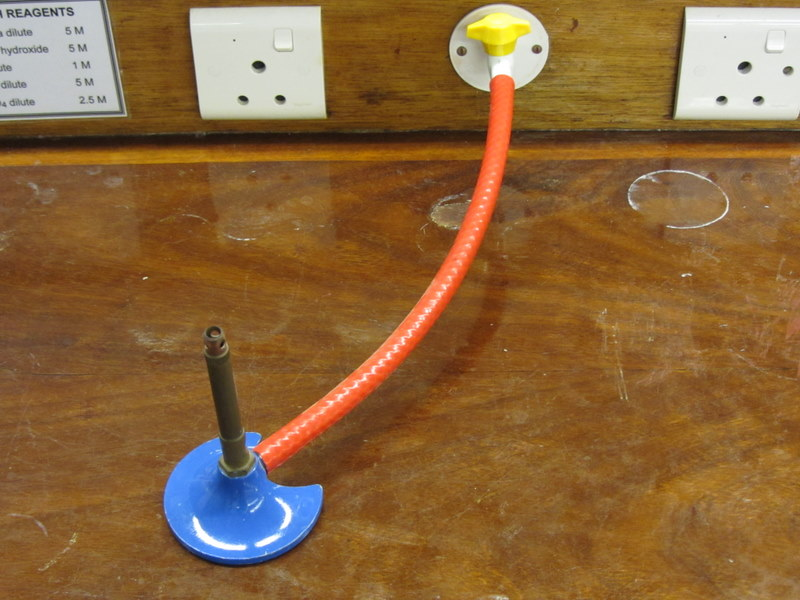
\includegraphics[width=.2\textwidth]{photos/bunsenburner.jpg} & \scalebox{.4}{\begin{pspicture}(-7.8,-1)(6.8,4)
\psset{dimen=middle,linewidth=0.053}%
% \psline[linewidth=0.05](0,5)(2,5)
% \psline[linewidth=0.04]{->}(1.7,4.5)(1,4.9)
% \uput[r](1.5,4.5){\large{toothpick with metal salt}}
\psframe(-1.25,0)(1.25,0.25)%
\psframe(-.5,1.25)(0.5,2.25)%
\multido{\n=-0.3+0.3}{3}{%
\pscircle(\n,1.75){0.1}}%
\psframe(-.25,2.25)(0.25,4.25)%
\psline(0.25,1.25)(0.25,0.5)(1.25,0.25)%
\psline(-1.25,0.25)(-.25,0.5)(-0.25,0.75)%
\psline(-2.25,0.75)(-.25,0.75)%
\psline(-2.25,1)(-.25,1)%
\psellipse(-.25,0.875)(0.1,0.125)%
\psframe[fillstyle=solid,linestyle=none](-2.25,0.75)(-0.25,1)%
\psline(-2.25,0.75)(-0.25,0.75)%
\psline(-2.25,1)(-0.25,1)(-.25,1.25)%
\pscurve(-0.25,0.5)(0,0.4)(0.25,0.5)
%flamme
\rput(0,4.25){%
\psclip{\psbezier[linestyle=none,fillstyle=gradient,gradmidpoint=0,%
gradbegin=OrangePale,gradend=yellow]%
(-0.25,0)(-0.35,0.5)(-0.4,0.75)%
(-0.35,1)(-0.25,1.5)(0.5,2)%
(0.25,1.5)(0.35,1)(0.4,0.75)%
(0.35,0.5)(0.25,0)(0,0)}%
\pspolygon[linestyle=none,fillstyle=gradient,gradmidpoint=0,gradbegin=cyan,gradend=white]%
(-0.25,0)(0.25,0)(0,1)%
\endpsclip}
\end{pspicture}} \\ \hline
Measuring cylinder & \includegraphics[width=.05\textheight]{photos/Measuring_cylinder_hannesgrobe_wikimedia.jpg} & \scalebox{.4}{\begin{pspicture}(0,0)(5,5) \pstEprouvette \end{pspicture}} \\ \hline
Pipette & 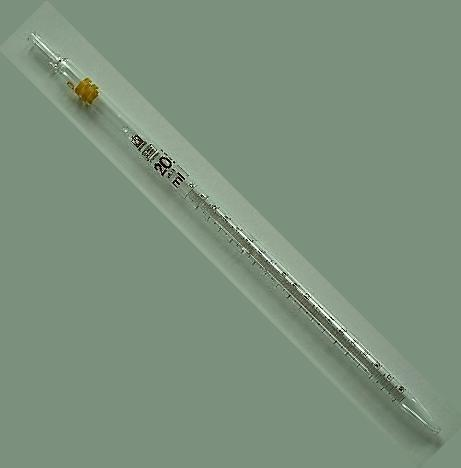
\includegraphics[width=.2\textwidth]{photos/Pipette.jpg} & \scalebox{.4}{\begin{pspicture}(0,0)(5,5) \pstpipette \end{pspicture}} \\ \hline
Watch glass & 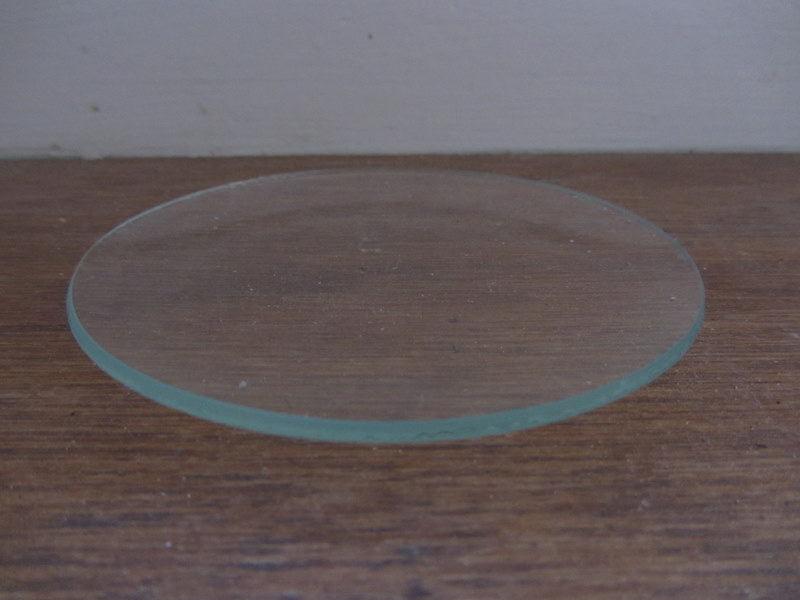
\includegraphics[width=.15\textwidth]{photos/watchglass.jpg} & \scalebox{.6} % Change this value to rescale the drawing.
{
\begin{pspicture}(0,-1.2576145)(1.8644192,-0.908)
\rput{-180.0}(2.32,0.0){\psarc[linewidth=0.04](1.16,0.0){1.16}{53.130104}{126.15819}}
\end{pspicture} 
}
 \\ \hline
% Mass meter & & \\ \hline
Thermometer & \includegraphics[width=.2\textwidth]{photos/thermometer.jpg} & \scalebox{.4} % Change this value to rescale the drawing.
{
\begin{pspicture}(0,-1.74)(0.52,1.76)
\psline[linewidth=0.04cm,doubleline=true,doublesep=0.12](0.3,1.72)(0.26,-1.44)
\psline[linewidth=0.04cm](0.22,1.7)(0.38,1.7)
\psbezier[linewidth=0.04](0.2,-1.38)(0.0,-1.62)(0.5,-1.72)(0.34,-1.38)
\end{pspicture} 
} \\ \hline
Funnel & 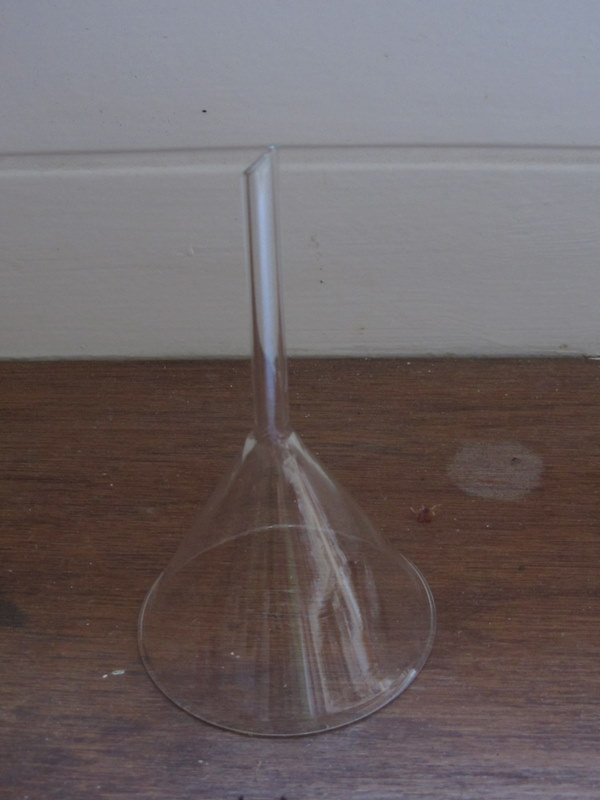
\includegraphics[width=.1\textwidth]{photos/funnel.jpg} & \scalebox{.4} % Change this value to rescale the drawing.
{
\begin{pspicture}(0,-1.17)(1.92,1.17)
\psline[linewidth=0.04cm](0.0,1.15)(0.88,0.21)
\psline[linewidth=0.04cm](1.0,0.25)(1.9,1.15)
\psline[linewidth=0.04cm,doubleline=true,doublesep=0.12](0.94,0.25)(0.94,-1.01)
\psline[linewidth=0.04cm](0.86,-0.97)(0.86,-1.15)
\end{pspicture} 
} \\ \hline
  \end{tabular} 
 \end{center}
\end{table}

The following image shows the correct setup for heating liquids on a Bunsen burner:\\
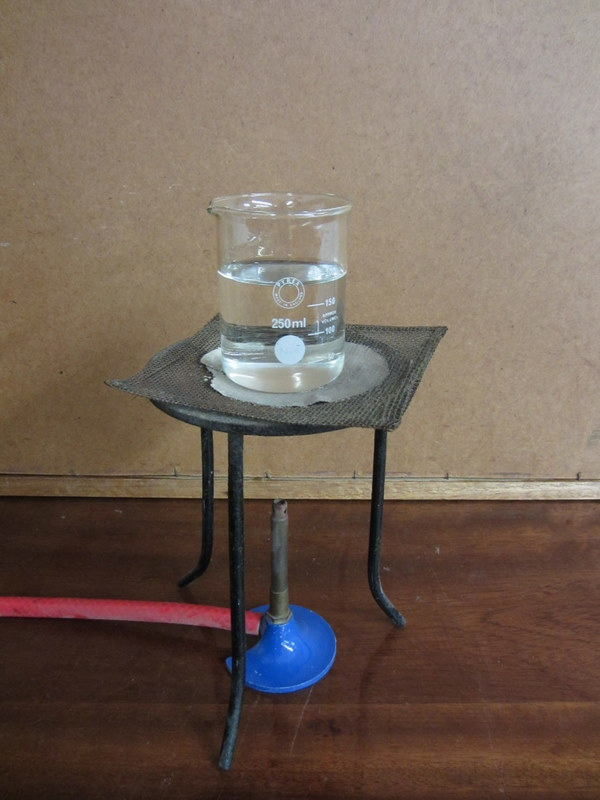
\includegraphics[width=.3\textwidth]{photos/beaker_tripod.jpg}\\
When reading any instrument (such as a measuring cylinder, a pipette, etc.) always make sure that the instrument is level and that your eye is at the level of the top of the liquid.

\subsection*{General safety rules}
            \nopagebreak
The following are some of the general guidelines and rules that you should always observe when working in a laboratory.
\begin{enumerate}[noitemsep, label=\textbf{\arabic*}. ] 
\item You are responsible for your own safety as well as the safety of others in the laboratory.
\item Do not eat or drink in the lab. Do not use lab glassware to eat or drink from.
\item Always behave responsibly in the lab. Do not run around or play practical jokes.
\item In case of accidents or chemical spills call your teacher at once.
\item Always check with your teacher how to dispose of waste. Chemicals should not be disposed of down the sink.
\item Only perform the experiments that your teacher instructs you to. Never mix chemicals for fun.
\item Never perform experiments alone. 
\item Always check the safety data of any chemicals you are going to use. 
\item Follow the given instructions exactly. Do not mix up steps or try things in a different order.
\item Be alert and careful when handling chemicals, hot glassware, etc.  
\item Ensure all Bunsen burners are turned off at the end of the practical and all chemical containers are sealed.
\item Never add water to acid. Always add the acid to water.
\item Never heat thick glassware as it will break. (i.e. do not heat measuring cylinders).
\item When you are smelling chemicals, place the container on a lab bench and use your hand to gently waft (fan) the vapours towards you.
\item Do not take chemicals from the lab.
\item Always work in a well ventilated room. Whenever you perform experiments, you should open the windows.
\item Do not leave Bunsen burners and flames unattended. 
\item Never smell, taste or touch chemicals unless instructed to do so.
\item Never point test tubes at people or yourself. When heating chemicals, always point the mouth of the test tube away from you and your classmates.
\end{enumerate}
\par 
\section{Hazard signs}
            \nopagebreak
The table below lists some of the common hazards signs that you may encounter. You should know what all of these mean.
\begin{table}[H]
 \begin{center}
  \begin{tabular}{|l|c|p{3cm}|l|c|p{3cm}|}\hline
   \textbf{Sign} & \textbf{Symbol} & \textbf{Meaning} & \textbf{Sign} & \textbf{Symbol} & \textbf{Meaning} \\ \hline
\parbox[c]{4em}{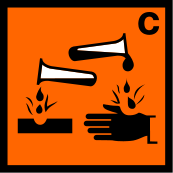
\includegraphics[width=.1\textwidth]{photos/corrosive.png}} & C & Corrosive. Chemicals with this label can burn your skin and eyes and burn holes in your clothes. An example is hydrochloric acid. & \parbox[c]{4em}{
\includegraphics[width=.1\textwidth]{photos/environment.png}} & N & Environmentally harmful. Chemicals with this label are damaging to the environment. An example is CFC's. \\ \hline 
\parbox[c]{4em}{
\includegraphics[width=.1\textwidth]{photos/explosive.png}} & E & Explosive. Chemicals with this label explode easily. An example is lead azide. & \parbox[c]{4em}{\includegraphics[width=.1\textwidth]{photos/flammable.png}} & F & Flammable. Chemicals with this label can catch fire easily. Example: methanol \\ \hline 
\parbox[c]{4em}{\includegraphics[width=.1\textwidth]{photos/harmful.png}} & Xn & Harmful. Chemicals labeled with this are generally considered to be damaging to humans. & \parbox[c]{4em}{
\includegraphics[width=.1\textwidth]{photos/irritant.png}} & Xi & Irritant. Chemicals with this label cause irritation to your eyes and skin. An example is hydrogen peroxide. \\ \hline 
\parbox[c]{4em}{\includegraphics[width=.1\textwidth]{photos/oxidise.png}} & O & Oxidizing. Chemicals with this label contain oxygen that may cause other materials to combust. An example is potassium dichromate. & \parbox[c]{4em}{\includegraphics[width=.1\textwidth]{photos/toxic.png}} & T & Toxic. Chemicals with this label are highly toxic. An example is mercury. \\ \hline 
  \end{tabular}
 \end{center}
\end{table}
\subsection*{Notes and information}
You can find safety data sheets at \textsl{http://www.msds.com/}. You should always look at these data sheets anytime you work with a new chemical. These data sheets contain information about how to work with chemicals and what dangers the chemicals pose to you and the environment. You should always try dispose of chemicals correctly and safely. Many chemicals cannot simply be washed down the sink. 

